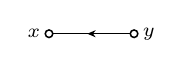
\begin{tikzpicture}[x=0.600cm, y=0.600cm, line width=0.550pt, baseline={([yshift=-0.6ex]0,0)}]
  \draw (0.900,0.000) -- (-0.900,0.000);
  \fill (-0.089,0.000) -- (0.089,-0.076) -- (0.031,0.000) -- (0.089,0.076) -- cycle;
  \draw[fill=white] (-0.900,0.000) circle (0.080);
  \draw[fill=white] (0.900,0.000) circle (0.080);
  \node[font=\scriptsize, inner sep=0pt, anchor=0] at (-1.070,0.000) {$x$};
  \node[font=\scriptsize, inner sep=0pt, anchor=180] at (1.070,0.000) {$y$};
\end{tikzpicture}
\allowbreak\;{-}\; 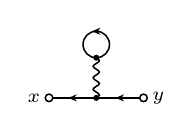
\begin{tikzpicture}[x=0.600cm, y=0.600cm, line width=0.550pt, baseline={([yshift=-0.6ex]0,0)}]
  \draw (0.000,0.000) -- (-1.000,0.000);
  \fill (-0.589,0.000) -- (-0.411,-0.076) -- (-0.469,0.000) -- (-0.411,0.076) -- cycle;
  \draw (1.000,0.000) -- (0.000,0.000);
  \fill (0.411,0.000) -- (0.589,-0.076) -- (0.531,0.000) -- (0.589,0.076) -- cycle;
  \draw plot[smooth, tension=0.7] coordinates {(0.000,0.850) (0.046,0.820) (0.066,0.789) (0.046,0.759) (0.000,0.729) (-0.046,0.698) (-0.066,0.668) (-0.046,0.638) (0.000,0.607) (0.046,0.577) (0.066,0.546) (0.046,0.516) (0.000,0.486) (-0.046,0.455) (-0.066,0.425) (-0.046,0.395) (0.000,0.364) (0.046,0.334) (0.066,0.304) (0.046,0.273) (0.000,0.243) (-0.046,0.213) (-0.066,0.182) (-0.046,0.152) (0.000,0.121) (0.046,0.091) (0.066,0.061) (0.046,0.030) (0.000,0.000)};
  \draw (0.000,0.850) arc[start angle=270.000, end angle=630.000, radius=0.280];
  \fill (-0.089,1.410) -- (0.089,1.334) -- (0.031,1.410) -- (0.089,1.486) -- cycle;
  \fill (0.000,0.850) circle (0.064);
  \fill (0.000,0.000) circle (0.064);
  \draw[fill=white] (-1.000,0.000) circle (0.080);
  \draw[fill=white] (1.000,0.000) circle (0.080);
  \node[font=\scriptsize, inner sep=0pt, anchor=0] at (-1.170,0.000) {$x$};
  \node[font=\scriptsize, inner sep=0pt, anchor=180] at (1.170,0.000) {$y$};
\end{tikzpicture}
\allowbreak\;{+}\; 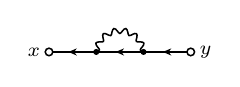
\begin{tikzpicture}[x=0.600cm, y=0.600cm, line width=0.550pt, baseline={([yshift=-0.6ex]0,0)}]
  \draw (-0.500,0.000) -- (-1.500,0.000);
  \fill (-1.089,0.000) -- (-0.911,-0.076) -- (-0.969,0.000) -- (-0.911,0.076) -- cycle;
  \draw (1.500,0.000) -- (0.500,0.000);
  \fill (0.911,0.000) -- (1.089,-0.076) -- (1.031,0.000) -- (1.089,0.076) -- cycle;
  \draw (0.500,0.000) -- (-0.500,0.000);
  \fill (-0.089,0.000) -- (0.089,-0.076) -- (0.031,0.000) -- (0.089,0.076) -- cycle;
  \draw plot[smooth, tension=0.7] coordinates {(0.500,0.000) (0.455,0.021) (0.433,0.043) (0.444,0.072) (0.476,0.110) (0.504,0.153) (0.507,0.188) (0.478,0.208) (0.427,0.213) (0.377,0.212) (0.348,0.222) (0.345,0.253) (0.357,0.301) (0.364,0.352) (0.352,0.385) (0.316,0.390) (0.269,0.372) (0.224,0.350) (0.193,0.347) (0.177,0.373) (0.167,0.422) (0.151,0.470) (0.126,0.495) (0.092,0.484) (0.057,0.447) (0.026,0.408) (0.000,0.391) (-0.026,0.408) (-0.057,0.447) (-0.092,0.484) (-0.126,0.495) (-0.151,0.470) (-0.167,0.422) (-0.177,0.373) (-0.193,0.347) (-0.224,0.350) (-0.269,0.372) (-0.316,0.390) (-0.352,0.385) (-0.364,0.352) (-0.357,0.301) (-0.345,0.253) (-0.348,0.222) (-0.377,0.212) (-0.427,0.213) (-0.478,0.208) (-0.507,0.188) (-0.504,0.153) (-0.476,0.110) (-0.444,0.072) (-0.433,0.043) (-0.455,0.021) (-0.500,0.000)};
  \fill (0.500,0.000) circle (0.064);
  \fill (-0.500,0.000) circle (0.064);
  \draw[fill=white] (-1.500,0.000) circle (0.080);
  \draw[fill=white] (1.500,0.000) circle (0.080);
  \node[font=\scriptsize, inner sep=0pt, anchor=0] at (-1.670,0.000) {$x$};
  \node[font=\scriptsize, inner sep=0pt, anchor=180] at (1.670,0.000) {$y$};
\end{tikzpicture}
\allowbreak\;{+}\; 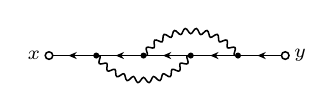
\begin{tikzpicture}[x=0.600cm, y=0.600cm, line width=0.550pt, baseline={([yshift=-0.6ex]0,0)}]
  \draw (-1.500,0.000) -- (-2.500,0.000);
  \fill (-2.089,0.000) -- (-1.911,-0.076) -- (-1.969,0.000) -- (-1.911,0.076) -- cycle;
  \draw (2.500,0.000) -- (1.500,0.000);
  \fill (1.911,0.000) -- (2.089,-0.076) -- (2.031,0.000) -- (2.089,0.076) -- cycle;
  \draw (-0.500,0.000) -- (-1.500,0.000);
  \fill (-1.089,0.000) -- (-0.911,-0.076) -- (-0.969,0.000) -- (-0.911,0.076) -- cycle;
  \draw (1.500,0.000) -- (0.500,0.000);
  \fill (0.911,0.000) -- (1.089,-0.076) -- (1.031,0.000) -- (1.089,0.076) -- cycle;
  \draw (0.500,0.000) -- (-0.500,0.000);
  \fill (-0.089,0.000) -- (0.089,-0.076) -- (0.031,0.000) -- (0.089,0.076) -- cycle;
  \draw plot[smooth, tension=0.7] coordinates {(1.500,0.000) (1.451,-0.002) (1.421,0.009) (1.418,0.041) (1.432,0.088) (1.444,0.137) (1.437,0.169) (1.405,0.179) (1.356,0.170) (1.308,0.159) (1.277,0.165) (1.268,0.195) (1.273,0.244) (1.276,0.294) (1.263,0.325) (1.230,0.329) (1.183,0.311) (1.138,0.292) (1.106,0.292) (1.092,0.320) (1.088,0.369) (1.082,0.419) (1.064,0.447) (1.031,0.444) (0.988,0.418) (0.947,0.391) (0.916,0.385) (0.896,0.410) (0.884,0.458) (0.869,0.506) (0.846,0.530) (0.814,0.521) (0.777,0.488) (0.741,0.454) (0.711,0.443) (0.688,0.464) (0.667,0.509) (0.644,0.553) (0.617,0.573) (0.586,0.558) (0.556,0.519) (0.527,0.479) (0.500,0.462) (0.473,0.479) (0.444,0.519) (0.414,0.558) (0.383,0.573) (0.356,0.553) (0.333,0.509) (0.312,0.464) (0.289,0.443) (0.259,0.454) (0.223,0.488) (0.186,0.521) (0.154,0.530) (0.131,0.506) (0.116,0.458) (0.104,0.410) (0.084,0.385) (0.053,0.391) (0.012,0.418) (-0.031,0.444) (-0.064,0.447) (-0.082,0.419) (-0.088,0.369) (-0.092,0.320) (-0.106,0.292) (-0.138,0.292) (-0.183,0.311) (-0.230,0.329) (-0.263,0.325) (-0.276,0.294) (-0.273,0.244) (-0.268,0.195) (-0.277,0.165) (-0.308,0.159) (-0.356,0.170) (-0.405,0.179) (-0.437,0.169) (-0.444,0.137) (-0.432,0.088) (-0.418,0.041) (-0.421,0.009) (-0.451,-0.002) (-0.500,0.000)};
  \draw plot[smooth, tension=0.7] coordinates {(-1.500,0.000) (-1.451,0.002) (-1.421,-0.009) (-1.418,-0.041) (-1.432,-0.088) (-1.444,-0.137) (-1.437,-0.169) (-1.405,-0.179) (-1.356,-0.170) (-1.308,-0.159) (-1.277,-0.165) (-1.268,-0.195) (-1.273,-0.244) (-1.276,-0.294) (-1.263,-0.325) (-1.230,-0.329) (-1.183,-0.311) (-1.138,-0.292) (-1.106,-0.292) (-1.092,-0.320) (-1.088,-0.369) (-1.082,-0.419) (-1.064,-0.447) (-1.031,-0.444) (-0.988,-0.418) (-0.947,-0.391) (-0.916,-0.385) (-0.896,-0.410) (-0.884,-0.458) (-0.869,-0.506) (-0.846,-0.530) (-0.814,-0.521) (-0.777,-0.488) (-0.741,-0.454) (-0.711,-0.443) (-0.688,-0.464) (-0.667,-0.509) (-0.644,-0.553) (-0.617,-0.573) (-0.586,-0.558) (-0.556,-0.519) (-0.527,-0.479) (-0.500,-0.462) (-0.473,-0.479) (-0.444,-0.519) (-0.414,-0.558) (-0.383,-0.573) (-0.356,-0.553) (-0.333,-0.509) (-0.312,-0.464) (-0.289,-0.443) (-0.259,-0.454) (-0.223,-0.488) (-0.186,-0.521) (-0.154,-0.530) (-0.131,-0.506) (-0.116,-0.458) (-0.104,-0.410) (-0.084,-0.385) (-0.053,-0.391) (-0.012,-0.418) (0.031,-0.444) (0.064,-0.447) (0.082,-0.419) (0.088,-0.369) (0.092,-0.320) (0.106,-0.292) (0.138,-0.292) (0.183,-0.311) (0.230,-0.329) (0.263,-0.325) (0.276,-0.294) (0.273,-0.244) (0.268,-0.195) (0.277,-0.165) (0.308,-0.159) (0.356,-0.170) (0.405,-0.179) (0.437,-0.169) (0.444,-0.137) (0.432,-0.088) (0.418,-0.041) (0.421,-0.009) (0.451,0.002) (0.500,0.000)};
  \fill (1.500,0.000) circle (0.064);
  \fill (-1.500,0.000) circle (0.064);
  \fill (0.500,0.000) circle (0.064);
  \fill (-0.500,0.000) circle (0.064);
  \draw[fill=white] (-2.500,0.000) circle (0.080);
  \draw[fill=white] (2.500,0.000) circle (0.080);
  \node[font=\scriptsize, inner sep=0pt, anchor=0] at (-2.670,0.000) {$x$};
  \node[font=\scriptsize, inner sep=0pt, anchor=180] at (2.670,0.000) {$y$};
\end{tikzpicture}
\allowbreak\;{-}\; 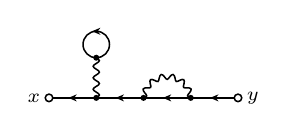
\begin{tikzpicture}[x=0.600cm, y=0.600cm, line width=0.550pt, baseline={([yshift=-0.6ex]0,0)}]
  \draw (-1.000,0.000) -- (-2.000,0.000);
  \fill (-1.589,0.000) -- (-1.411,-0.076) -- (-1.469,0.000) -- (-1.411,0.076) -- cycle;
  \draw (2.000,0.000) -- (1.000,0.000);
  \fill (1.411,0.000) -- (1.589,-0.076) -- (1.531,0.000) -- (1.589,0.076) -- cycle;
  \draw (0.000,0.000) -- (-1.000,0.000);
  \fill (-0.589,0.000) -- (-0.411,-0.076) -- (-0.469,0.000) -- (-0.411,0.076) -- cycle;
  \draw (1.000,0.000) -- (0.000,0.000);
  \fill (0.411,0.000) -- (0.589,-0.076) -- (0.531,0.000) -- (0.589,0.076) -- cycle;
  \draw plot[smooth, tension=0.7] coordinates {(1.000,0.000) (0.955,0.021) (0.933,0.043) (0.944,0.072) (0.976,0.110) (1.004,0.153) (1.007,0.188) (0.978,0.208) (0.927,0.213) (0.877,0.212) (0.848,0.222) (0.845,0.253) (0.857,0.301) (0.864,0.352) (0.852,0.385) (0.816,0.390) (0.769,0.372) (0.724,0.350) (0.693,0.347) (0.677,0.373) (0.667,0.422) (0.651,0.470) (0.626,0.495) (0.592,0.484) (0.557,0.447) (0.526,0.408) (0.500,0.391) (0.474,0.408) (0.443,0.447) (0.408,0.484) (0.374,0.495) (0.349,0.470) (0.333,0.422) (0.323,0.373) (0.307,0.347) (0.276,0.350) (0.231,0.372) (0.184,0.390) (0.148,0.385) (0.136,0.352) (0.143,0.301) (0.155,0.253) (0.152,0.222) (0.123,0.212) (0.073,0.213) (0.022,0.208) (-0.007,0.188) (-0.004,0.153) (0.024,0.110) (0.056,0.072) (0.067,0.043) (0.045,0.021) (0.000,0.000)};
  \draw plot[smooth, tension=0.7] coordinates {(-1.000,0.850) (-0.954,0.820) (-0.934,0.789) (-0.954,0.759) (-1.000,0.729) (-1.046,0.698) (-1.066,0.668) (-1.046,0.638) (-1.000,0.607) (-0.954,0.577) (-0.934,0.546) (-0.954,0.516) (-1.000,0.486) (-1.046,0.455) (-1.066,0.425) (-1.046,0.395) (-1.000,0.364) (-0.954,0.334) (-0.934,0.304) (-0.954,0.273) (-1.000,0.243) (-1.046,0.213) (-1.066,0.182) (-1.046,0.152) (-1.000,0.121) (-0.954,0.091) (-0.934,0.061) (-0.954,0.030) (-1.000,0.000)};
  \draw (-1.000,0.850) arc[start angle=270.000, end angle=630.000, radius=0.280];
  \fill (-1.089,1.410) -- (-0.911,1.334) -- (-0.969,1.410) -- (-0.911,1.486) -- cycle;
  \fill (-1.000,0.850) circle (0.064);
  \fill (1.000,0.000) circle (0.064);
  \fill (-1.000,0.000) circle (0.064);
  \fill (0.000,0.000) circle (0.064);
  \draw[fill=white] (-2.000,0.000) circle (0.080);
  \draw[fill=white] (2.000,0.000) circle (0.080);
  \node[font=\scriptsize, inner sep=0pt, anchor=0] at (-2.170,0.000) {$x$};
  \node[font=\scriptsize, inner sep=0pt, anchor=180] at (2.170,0.000) {$y$};
\end{tikzpicture}
\allowbreak\;{+}\; 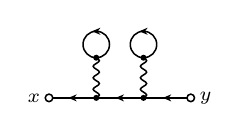
\begin{tikzpicture}[x=0.600cm, y=0.600cm, line width=0.550pt, baseline={([yshift=-0.6ex]0,0)}]
  \draw (-0.500,0.000) -- (-1.500,0.000);
  \fill (-1.089,0.000) -- (-0.911,-0.076) -- (-0.969,0.000) -- (-0.911,0.076) -- cycle;
  \draw (1.500,0.000) -- (0.500,0.000);
  \fill (0.911,0.000) -- (1.089,-0.076) -- (1.031,0.000) -- (1.089,0.076) -- cycle;
  \draw (0.500,0.000) -- (-0.500,0.000);
  \fill (-0.089,0.000) -- (0.089,-0.076) -- (0.031,0.000) -- (0.089,0.076) -- cycle;
  \draw plot[smooth, tension=0.7] coordinates {(0.500,0.850) (0.546,0.820) (0.566,0.789) (0.546,0.759) (0.500,0.729) (0.454,0.698) (0.434,0.668) (0.454,0.638) (0.500,0.607) (0.546,0.577) (0.566,0.546) (0.546,0.516) (0.500,0.486) (0.454,0.455) (0.434,0.425) (0.454,0.395) (0.500,0.364) (0.546,0.334) (0.566,0.304) (0.546,0.273) (0.500,0.243) (0.454,0.213) (0.434,0.182) (0.454,0.152) (0.500,0.121) (0.546,0.091) (0.566,0.061) (0.546,0.030) (0.500,0.000)};
  \draw plot[smooth, tension=0.7] coordinates {(-0.500,0.850) (-0.454,0.820) (-0.434,0.789) (-0.454,0.759) (-0.500,0.729) (-0.546,0.698) (-0.566,0.668) (-0.546,0.638) (-0.500,0.607) (-0.454,0.577) (-0.434,0.546) (-0.454,0.516) (-0.500,0.486) (-0.546,0.455) (-0.566,0.425) (-0.546,0.395) (-0.500,0.364) (-0.454,0.334) (-0.434,0.304) (-0.454,0.273) (-0.500,0.243) (-0.546,0.213) (-0.566,0.182) (-0.546,0.152) (-0.500,0.121) (-0.454,0.091) (-0.434,0.061) (-0.454,0.030) (-0.500,0.000)};
  \draw (0.500,0.850) arc[start angle=270.000, end angle=630.000, radius=0.280];
  \fill (0.411,1.410) -- (0.589,1.334) -- (0.531,1.410) -- (0.589,1.486) -- cycle;
  \draw (-0.500,0.850) arc[start angle=270.000, end angle=630.000, radius=0.280];
  \fill (-0.589,1.410) -- (-0.411,1.334) -- (-0.469,1.410) -- (-0.411,1.486) -- cycle;
  \fill (0.500,0.850) circle (0.064);
  \fill (-0.500,0.850) circle (0.064);
  \fill (0.500,0.000) circle (0.064);
  \fill (-0.500,0.000) circle (0.064);
  \draw[fill=white] (-1.500,0.000) circle (0.080);
  \draw[fill=white] (1.500,0.000) circle (0.080);
  \node[font=\scriptsize, inner sep=0pt, anchor=0] at (-1.670,0.000) {$x$};
  \node[font=\scriptsize, inner sep=0pt, anchor=180] at (1.670,0.000) {$y$};
\end{tikzpicture}
\allowbreak\;{+}\; 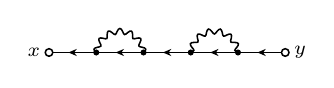
\begin{tikzpicture}[x=0.600cm, y=0.600cm, line width=0.550pt, baseline={([yshift=-0.6ex]0,0)}]
  \draw (-1.500,0.000) -- (-2.500,0.000);
  \fill (-2.089,0.000) -- (-1.911,-0.076) -- (-1.969,0.000) -- (-1.911,0.076) -- cycle;
  \draw (2.500,0.000) -- (1.500,0.000);
  \fill (1.911,0.000) -- (2.089,-0.076) -- (2.031,0.000) -- (2.089,0.076) -- cycle;
  \draw (-0.500,0.000) -- (-1.500,0.000);
  \fill (-1.089,0.000) -- (-0.911,-0.076) -- (-0.969,0.000) -- (-0.911,0.076) -- cycle;
  \draw plot[smooth, tension=0.7] coordinates {(-1.500,0.000) (-1.537,0.035) (-1.548,0.069) (-1.524,0.095) (-1.476,0.110) (-1.427,0.121) (-1.401,0.138) (-1.405,0.168) (-1.427,0.213) (-1.445,0.260) (-1.441,0.296) (-1.407,0.308) (-1.357,0.301) (-1.308,0.290) (-1.278,0.293) (-1.268,0.322) (-1.269,0.372) (-1.265,0.423) (-1.245,0.453) (-1.209,0.450) (-1.167,0.422) (-1.128,0.390) (-1.099,0.380) (-1.078,0.402) (-1.057,0.447) (-1.031,0.491) (-1.000,0.509) (-0.969,0.491) (-0.943,0.447) (-0.922,0.402) (-0.901,0.380) (-0.872,0.390) (-0.833,0.422) (-0.791,0.450) (-0.755,0.453) (-0.735,0.423) (-0.731,0.372) (-0.732,0.322) (-0.722,0.293) (-0.692,0.290) (-0.643,0.301) (-0.593,0.308) (-0.559,0.296) (-0.555,0.260) (-0.573,0.213) (-0.595,0.168) (-0.599,0.138) (-0.573,0.121) (-0.524,0.110) (-0.476,0.095) (-0.452,0.069) (-0.463,0.035) (-0.500,0.000)};
  \draw (1.500,0.000) -- (0.500,0.000);
  \fill (0.911,0.000) -- (1.089,-0.076) -- (1.031,0.000) -- (1.089,0.076) -- cycle;
  \draw plot[smooth, tension=0.7] coordinates {(1.500,0.000) (1.455,0.021) (1.433,0.043) (1.444,0.072) (1.476,0.110) (1.504,0.153) (1.507,0.188) (1.478,0.208) (1.427,0.213) (1.377,0.212) (1.348,0.222) (1.345,0.253) (1.357,0.301) (1.364,0.352) (1.352,0.385) (1.316,0.390) (1.269,0.372) (1.224,0.350) (1.193,0.347) (1.177,0.373) (1.167,0.422) (1.151,0.470) (1.126,0.495) (1.092,0.484) (1.057,0.447) (1.026,0.408) (1.000,0.391) (0.974,0.408) (0.943,0.447) (0.908,0.484) (0.874,0.495) (0.849,0.470) (0.833,0.422) (0.823,0.373) (0.807,0.347) (0.776,0.350) (0.731,0.372) (0.684,0.390) (0.648,0.385) (0.636,0.352) (0.643,0.301) (0.655,0.253) (0.652,0.222) (0.623,0.212) (0.573,0.213) (0.522,0.208) (0.493,0.188) (0.496,0.153) (0.524,0.110) (0.556,0.072) (0.567,0.043) (0.545,0.021) (0.500,0.000)};
  \draw (0.500,0.000) -- (-0.500,0.000);
  \fill (-0.089,0.000) -- (0.089,-0.076) -- (0.031,0.000) -- (0.089,0.076) -- cycle;
  \fill (1.500,0.000) circle (0.064);
  \fill (-1.500,0.000) circle (0.064);
  \fill (0.500,0.000) circle (0.064);
  \fill (-0.500,0.000) circle (0.064);
  \draw[fill=white] (-2.500,0.000) circle (0.080);
  \draw[fill=white] (2.500,0.000) circle (0.080);
  \node[font=\scriptsize, inner sep=0pt, anchor=0] at (-2.670,0.000) {$x$};
  \node[font=\scriptsize, inner sep=0pt, anchor=180] at (2.670,0.000) {$y$};
\end{tikzpicture}
\allowbreak\;{-}\; 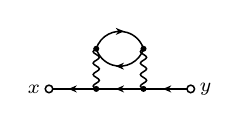
\begin{tikzpicture}[x=0.600cm, y=0.600cm, line width=0.550pt, baseline={([yshift=-0.6ex]0,0)}]
  \draw (-0.500,0.000) -- (-1.500,0.000);
  \fill (-1.089,0.000) -- (-0.911,-0.076) -- (-0.969,0.000) -- (-0.911,0.076) -- cycle;
  \draw (1.500,0.000) -- (0.500,0.000);
  \fill (0.911,0.000) -- (1.089,-0.076) -- (1.031,0.000) -- (1.089,0.076) -- cycle;
  \draw (0.500,0.000) -- (-0.500,0.000);
  \fill (-0.089,0.000) -- (0.089,-0.076) -- (0.031,0.000) -- (0.089,0.076) -- cycle;
  \draw (-0.500,0.850) arc[start angle=162.811, end angle=17.189, radius=0.523];
  \fill (0.089,1.219) -- (-0.089,1.294) -- (-0.031,1.219) -- (-0.089,1.143) -- cycle;
  \draw (0.500,0.850) arc[start angle=342.811, end angle=197.189, radius=0.523];
  \fill (-0.089,0.481) -- (0.089,0.406) -- (0.031,0.481) -- (0.089,0.557) -- cycle;
  \draw plot[smooth, tension=0.7] coordinates {(0.500,0.000) (0.454,0.030) (0.434,0.061) (0.454,0.091) (0.500,0.121) (0.546,0.152) (0.566,0.182) (0.546,0.212) (0.500,0.243) (0.454,0.273) (0.434,0.304) (0.454,0.334) (0.500,0.364) (0.546,0.395) (0.566,0.425) (0.546,0.455) (0.500,0.486) (0.454,0.516) (0.434,0.546) (0.454,0.577) (0.500,0.607) (0.546,0.638) (0.566,0.668) (0.546,0.698) (0.500,0.729) (0.454,0.759) (0.434,0.789) (0.454,0.820) (0.500,0.850)};
  \draw plot[smooth, tension=0.7] coordinates {(-0.500,0.000) (-0.546,0.030) (-0.566,0.061) (-0.546,0.091) (-0.500,0.121) (-0.454,0.152) (-0.434,0.182) (-0.454,0.212) (-0.500,0.243) (-0.546,0.273) (-0.566,0.304) (-0.546,0.334) (-0.500,0.364) (-0.454,0.395) (-0.434,0.425) (-0.454,0.455) (-0.500,0.486) (-0.546,0.516) (-0.566,0.546) (-0.546,0.577) (-0.500,0.607) (-0.454,0.638) (-0.434,0.668) (-0.454,0.698) (-0.500,0.729) (-0.546,0.759) (-0.566,0.789) (-0.546,0.820) (-0.500,0.850)};
  \fill (0.500,0.000) circle (0.064);
  \fill (-0.500,0.000) circle (0.064);
  \fill (0.500,0.850) circle (0.064);
  \fill (-0.500,0.850) circle (0.064);
  \draw[fill=white] (-1.500,0.000) circle (0.080);
  \draw[fill=white] (1.500,0.000) circle (0.080);
  \node[font=\scriptsize, inner sep=0pt, anchor=0] at (-1.670,0.000) {$x$};
  \node[font=\scriptsize, inner sep=0pt, anchor=180] at (1.670,0.000) {$y$};
\end{tikzpicture}
\allowbreak\;{-}\; 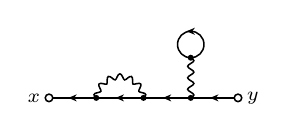
\begin{tikzpicture}[x=0.600cm, y=0.600cm, line width=0.550pt, baseline={([yshift=-0.6ex]0,0)}]
  \draw (-1.000,0.000) -- (-2.000,0.000);
  \fill (-1.589,0.000) -- (-1.411,-0.076) -- (-1.469,0.000) -- (-1.411,0.076) -- cycle;
  \draw (2.000,0.000) -- (1.000,0.000);
  \fill (1.411,0.000) -- (1.589,-0.076) -- (1.531,0.000) -- (1.589,0.076) -- cycle;
  \draw (0.000,0.000) -- (-1.000,0.000);
  \fill (-0.589,0.000) -- (-0.411,-0.076) -- (-0.469,0.000) -- (-0.411,0.076) -- cycle;
  \draw plot[smooth, tension=0.7] coordinates {(-1.000,0.000) (-1.037,0.035) (-1.048,0.069) (-1.024,0.095) (-0.976,0.110) (-0.927,0.121) (-0.901,0.138) (-0.905,0.168) (-0.927,0.213) (-0.945,0.260) (-0.941,0.296) (-0.907,0.308) (-0.857,0.301) (-0.808,0.290) (-0.778,0.293) (-0.768,0.322) (-0.769,0.372) (-0.765,0.423) (-0.745,0.453) (-0.709,0.450) (-0.667,0.422) (-0.628,0.390) (-0.599,0.380) (-0.578,0.402) (-0.557,0.447) (-0.531,0.491) (-0.500,0.509) (-0.469,0.491) (-0.443,0.447) (-0.422,0.402) (-0.401,0.380) (-0.372,0.390) (-0.333,0.422) (-0.291,0.450) (-0.255,0.453) (-0.235,0.423) (-0.231,0.372) (-0.232,0.322) (-0.222,0.293) (-0.192,0.290) (-0.143,0.301) (-0.093,0.308) (-0.059,0.296) (-0.055,0.260) (-0.073,0.213) (-0.095,0.168) (-0.099,0.138) (-0.073,0.121) (-0.024,0.110) (0.024,0.095) (0.048,0.069) (0.037,0.035) (0.000,0.000)};
  \draw (1.000,0.000) -- (0.000,0.000);
  \fill (0.411,0.000) -- (0.589,-0.076) -- (0.531,0.000) -- (0.589,0.076) -- cycle;
  \draw plot[smooth, tension=0.7] coordinates {(1.000,0.850) (1.046,0.820) (1.066,0.789) (1.046,0.759) (1.000,0.729) (0.954,0.698) (0.934,0.668) (0.954,0.638) (1.000,0.607) (1.046,0.577) (1.066,0.546) (1.046,0.516) (1.000,0.486) (0.954,0.455) (0.934,0.425) (0.954,0.395) (1.000,0.364) (1.046,0.334) (1.066,0.304) (1.046,0.273) (1.000,0.243) (0.954,0.213) (0.934,0.182) (0.954,0.152) (1.000,0.121) (1.046,0.091) (1.066,0.061) (1.046,0.030) (1.000,0.000)};
  \draw (1.000,0.850) arc[start angle=270.000, end angle=630.000, radius=0.280];
  \fill (0.911,1.410) -- (1.089,1.334) -- (1.031,1.410) -- (1.089,1.486) -- cycle;
  \fill (1.000,0.850) circle (0.064);
  \fill (1.000,0.000) circle (0.064);
  \fill (-1.000,0.000) circle (0.064);
  \fill (0.000,0.000) circle (0.064);
  \draw[fill=white] (-2.000,0.000) circle (0.080);
  \draw[fill=white] (2.000,0.000) circle (0.080);
  \node[font=\scriptsize, inner sep=0pt, anchor=0] at (-2.170,0.000) {$x$};
  \node[font=\scriptsize, inner sep=0pt, anchor=180] at (2.170,0.000) {$y$};
\end{tikzpicture}